%%%%%%%%%%%%%%%%%%%%%%%%%%%%%%%%%%%%%%%%%%
% Mathematics Final Year Research Projects
% LaTeX Template
% Version 1.0 (31/01/24)
%
% This template has been adapted from: https://www.overleaf.com/latex/templates/imperial-college-report-template/wncnzptkhnbc
% Students should feel free to adapt this template to their needs.
%%%%%%%%%%%%%%%%%%%%%%%%%%%%%%%%%%%%%%%%%%
%----------------------------------------------------------------------------------------
% PACKAGES AND OTHER DOCUMENT CONFIGURATIONS
%----------------------------------------------------------------------------------------
\documentclass[a4paper,11pt, titlepage]{article}

%% Language and font encodings
\usepackage[english]{babel}
\usepackage[utf8]{inputenc}
\usepackage[T1]{fontenc}

%% Sets page size and margins
\usepackage[a4paper,top=1in,bottom=1in,left=1in,right=1in,marginparwidth=1.75cm]{geometry}

%% Useful packages
\usepackage{afterpage}
\usepackage{amsmath}
\usepackage{amsthm}
\usepackage{amssymb}
\usepackage{csquotes}
\usepackage{enumitem}
\usepackage{graphicx}
\usepackage{lipsum}
\usepackage{booktabs}

% Listings (for displaying code):
\usepackage{listings}
\lstset{
    frame = single, 
    framexleftmargin=15pt
}

% Center figure captions:
\usepackage{caption}
\captionsetup[figure]{labelfont={bf},name={Figure},labelsep=quad}
\captionsetup[table]{labelfont={bf},name={Table},labelsep=quad}


% ----------- Algorithm2e setup
\usepackage[ruled,vlined]{algorithm2e}
\makeatletter
\renewcommand{\SetKwInOut}[2]{%
  \sbox\algocf@inoutbox{\KwSty{#2}\algocf@typo:}%
  \expandafter\ifx\csname InOutSizeDefined\endcsname\relax% if first time used
    \newcommand\InOutSizeDefined{}\setlength{\inoutsize}{\wd\algocf@inoutbox}%
    \sbox\algocf@inoutbox{\parbox[t]{\inoutsize}{\KwSty{#2}\algocf@typo:\hfill}~}\setlength{\inoutindent}{\wd\algocf@inoutbox}%
  \else% else keep the larger dimension
    \ifdim\wd\algocf@inoutbox>\inoutsize%
    \setlength{\inoutsize}{\wd\algocf@inoutbox}%
    \sbox\algocf@inoutbox{\parbox[t]{\inoutsize}{\KwSty{#2}\algocf@typo:\hfill}~}\setlength{\inoutindent}{\wd\algocf@inoutbox}%
    \fi%
  \fi% the dimension of the box is now defined.
  \algocf@newcommand{#1}[1]{%
    \ifthenelse{\boolean{algocf@inoutnumbered}}{\relax}{\everypar={\relax}}%
%     {\let\\\algocf@newinout\hangindent=\wd\algocf@inoutbox\hangafter=1\parbox[t]{\inoutsize}{\KwSty{#2}\algocf@typo\hfill:}~##1\par}%
    {\let\\\algocf@newinout\hangindent=\inoutindent\hangafter=1\parbox[t]{\inoutsize}{\KwSty{#2}\algocf@typo:\hfill}~##1\par}%
    \algocf@linesnumbered% reset the numbering of the lines
  }}%
\makeatother
% --------- end algorithm2e setup

% \bm allows typing bold math:
\usepackage{bm}
\usepackage[normalem]{ulem}

\usepackage[colorinlistoftodos]{todonotes}
\usepackage[colorlinks=true, allcolors=blue]{hyperref}

\renewcommand*{\rmdefault}{bch}
\renewcommand*{\ttdefault}{lmtt}
\newcommand{\citationneeded}{\textcolor{red}{[citation-needed]}}

\DeclareMathOperator*{\argmin}{\arg\!\min}
\DeclareMathOperator*{\argmax}{\arg\!\max}

% Add bigger skip between paragraphs, makes reading easier:
\setlength{\parskip}{0.5em}

% Bibliography
\usepackage[numbers, comma, square, sort&compress]{natbib}
\bibliographystyle{abbrvunsrtnat.bst}


% Theorem, Lemma, Corollary and Proofs
\theoremstyle{definition}
\newtheorem{definition}{Definition}[section]
\theoremstyle{plain}
\newtheorem{theorem}{Theorem}[section]
\newtheorem{corollary}{Corollary}[theorem]
\newtheorem{lemma}[theorem]{Lemma}
\theoremstyle{remark}
\newtheorem*{remark}{Remark}

%----------------------------------------------------------------------------------------
% END OF DOCUMENT CONFIGURATION
%----------------------------------------------------------------------------------------

%----------------------------------------------------------------------------------------
% IMPORTANT INFORMATION TO MODIFY FOR THE TITLE PAGE
%----------------------------------------------------------------------------------------
\newcommand{\reporttitle}{Scientific Machine Learning} % Title of your research project
\newcommand{\reportauthorA}{James Tay (CID: 02015786)} % First Name, Last Name and CID of student 1
\newcommand{\reportauthorB}{Student name 2 (CID: -------------)} % First Name, Last Name and CID of student 2
\newcommand{\reportauthorC}{Student name 3 (CID: -------------)} % First Name, Last Name and CID of student 3
\newcommand{\reportauthorD}{Student name 4 (CID: -------------)} % First Name, Last Name and CID of student 4
\newcommand{\reportauthorE}{Student name 5 (CID: -------------)} % First Name, Last Name and CID of student 5
\newcommand{\supervisor}{Sheehan Olver} % First Name and Last Name of your supervisor(s)
%----------------------------------------------------------------------------------------

%----------------------------------------------------------------------------------------
% To compile this file, use the following sequence: 
%	latex main.tex
%	bibtex main.tex
%	latex main.tex
%	latex main.tex
%----------------------------------------------------------------------------------------

%----------------------------------------------------------------------------------------
% START OF DOCUMENT
%----------------------------------------------------------------------------------------
\begin{document}

%%%%%%%%%%%%%%%%%%%%%%%%%%%%%%%%%%%%%
% Title page
%%%%%%%%%%%%%%%%%%%%%%%%%%%%%%%%%%%%%
\begin{titlepage}
\newcommand{\HRule}{\rule{\linewidth}{0.5mm}} % Defines a new command for the horizontal lines, change thickness here
%----------------------------------------------------------------------------------------
%	LOGO SECTION
%----------------------------------------------------------------------------------------

\includegraphics[width=8cm]{Imperial_logo.png}\\[1cm] % Include a department/university logo - this will require the graphicx package
%----------------------------------------------------------------------------------------
\center % Center everything on the page
%----------------------------------------------------------------------------------------
%	HEADING SECTIONS
%----------------------------------------------------------------------------------------
% For M3R or M4R reports, comment out as appropriate
\textsc{\LARGE Imperial College London}\\[0.5cm] 
\textsc{\Large Department of Mathematics}\\[1.5cm] 
\textsc{\Large Second-year Group Research Project}\\[0.5cm]
%----------------------------------------------------------------------------------------
%	TITLE SECTION
%----------------------------------------------------------------------------------------
\makeatletter
\HRule \\[0.6cm]
{ \huge \bfseries \reporttitle}\\[0.6cm] % Title of your document
\HRule \\[1.5cm]
%----------------------------------------------------------------------------------------
%	AUTHOR SECTION
%----------------------------------------------------------------------------------------
\begin{minipage}{0.4\textwidth}
\begin{flushleft} \large
\emph{Author:}\\
\reportauthorA \\
\reportauthorB \\
\reportauthorC \\
\reportauthorD \\
\reportauthorE
\end{flushleft}
\end{minipage}
~
\begin{minipage}{0.4\textwidth}
\begin{flushright} \large
\emph{Supervisor(s):} \\
\supervisor % Supervisor's name
\end{flushright}
\end{minipage}\\[2cm]
\makeatother
%----------------------------------------------------------------------------------------
%	FOOTER & DATE SECTION
%----------------------------------------------------------------------------------------
\vfill
\makeatletter
{\large \today}\\[2cm] % Date, change the \today to a set date if you want to be precise
\makeatother
\end{titlepage}
%%%%%%%%%%%%%%%%%%%%%%%%%%%%%%%%%%%%%

%%%%%%%%%%%%%%%%%%%%%%%%%%%%%%%%%%%%%
% Abstract
\begin{abstract}
Type your abstract here. The abstract is a summary of the contents of the project. It should be brief but informative, and
should avoid technicalities as far as possible.
\end{abstract}
%%%%%%%%%%%%%%%%%%%%%%%%%%%%%%%%%%%%%
 
%%%%%%%%%%%%%%%%%%%%%%%%%%%%%%%%%%%%%
% Table of contents
\tableofcontents
\clearpage
%%%%%%%%%%%%%%%%%%%%%%%%%%%%%%%%%%%%%

%%%%%%%%%%%%%%%%%%%%%%%%%%%%%%%%%%%%%
% Main sections
%%%%%%%%%%%%%%%%%%%%%%%%%%%%%%%%%%%%%
\section{Introduction}
\label{sec:introduction}

The introduction should attempt to set your work in the context of other work done in the field. It
should demonstrate that you are aware of what you are doing, and how it relates to other work
(with references). It should also provide an overview of the contents of the project. You should
highlight your individual contributions and any novel result: which of the calculations, theorems,
examples, proofs, conjectures, codes etc. are your own?

\section{Examples}

Here is a section with a few useful examples. 

\begin{figure}[b!] %Use h,t,b,! to enforce the location of the figure
    \centering
    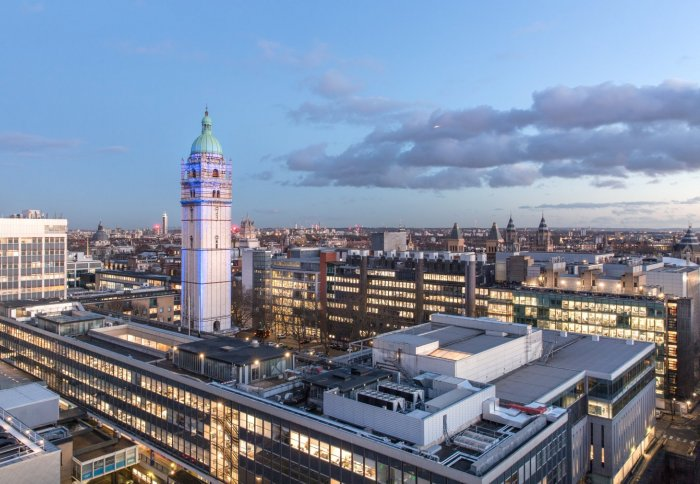
\includegraphics[width=0.8\textwidth]{figures/imperial.jpg}
    \caption{This is an example of how you include a figure with a descriptive caption. This is an image of the South Kensington campus of Imperial College London on which we can recognize Queen's tower.}
    \label{fig:imperial-picture}
\end{figure}

Here is some filler text to show you what a few pages may look like. \lipsum[2-4] See Figure \ref{fig:imperial-picture}. \textbf{This is how you reference your figure in the text.}

\begin{table}[]
    \centering
    \begin{tabular}{llr}  
        \toprule
        \multicolumn{2}{c}{Module} \\
        \cmidrule(r){1-2}
        Module code    & Module name & Number of students \\
        \midrule
              & per gram    & 13.65      \\
                      &    each     & 0.01       \\
        Gnu       & stuffed     & 92.50      \\
        Emu       & stuffed     & 33.33      \\
        Armadillo & frozen      & 8.99       \\
        \bottomrule
    \end{tabular}
    \caption{Example booktabs table. Booktabs tables are nicer than regular ones. This site has a nice GUI for making LaTeX tables, and has a Booktabs option: https://www.tablesgenerator.com/}
    \label{tab:my_label}
\end{table}

\lipsum[1-4] \textbf{This is how you would reference a table:} Table \ref{tab:my_label}. 

\subsection{Section Example}
\label{sec:sec_example}
\lipsum[1]
\subsubsection{Subsection Example}
\label{sec:subsec_example}
\lipsum[1]

Note that you can reference chapters, sections, subsections and subsubsections. For example: Subsection \ref{sec:subsec_example}!

\subsection{Math Example}

While math can be written inline like so $f(x) = \sum_{n=0}^{\infty} \frac{x^n}{n!}$, we often need to write stand-alone equations like so
\begin{equation}
\textrm{score}(x) = \left(\lambda_m\sum_{i=0}^{|\mathbf{m}|} \log \hat{p}_m(d(x, \mathbf{m}_i) \mid l_i)\right) + \left(\lambda_l\sum_{i=0}^{|\mathbf{l}|} \log\hat{p}_l(d(x, \mathbf{l}_i) \mid \mathbf{v}_i)\right) + \lambda_p \hat{p}_p(x)
\end{equation}

To write equations over multiple lines (like systems of equation or equations too long to fit the page), one can use the \textit{align} environment coupled to the \textit{subequations} environment like so
\begin{subequations}
\begin{align}
    \mathbb{P}(0 \leadsto -a) &= D\int_0^\infty dt\, k_r e^{-k_r t}\int_0^t d\tau\,\partial_x u \big|_{x=-a}, \\
    \mathbb{P}(0 \leadsto b) &= -D\int_0^\infty dt\, k_r e^{-k_r t}\int_0^t d\tau\,\partial_x u \big|_{x=b}.
\end{align}
\end{subequations}

\subsection{Theorem and Proofs}

This section is directly taken from \href{https://www.overleaf.com/learn/latex/Theorems_and_proofs}{Overleaf}. Please do consult the webpage for more information and discuss with your supervisors. 

Theorems can easily be defined:

\begin{theorem}
Let \(f\) be a function whose derivative exists in every point, then \(f\) is 
a continuous function.
\end{theorem}

\begin{theorem}[Pythagorean theorem]
\label{pythagorean}
This is a theorem about right triangles and can be summarised in the next 
equation 
\[ x^2 + y^2 = z^2 \]
\end{theorem}

And a consequence of theorem \ref{pythagorean} is the statement in the next 
corollary.

\begin{corollary}
There's no right rectangle whose sides measure 3cm, 4cm, and 6cm.
\end{corollary}

You can reference theorems such as \ref{pythagorean} when a label is assigned.

\begin{lemma}
Given two line segments whose lengths are \(a\) and \(b\) respectively there is a 
real number \(r\) such that \(b=ra\).
\end{lemma}

As you can see, theorems, corollaries and lemmas are italicised. Often, definitions are not: 
\begin{definition}[Fibration]
A fibration is a mapping between two topological spaces that has the homotopy lifting property for every space \(X\).
\end{definition}
This can be changed using the \verb!\theoremstyle{}! command in the preamble. 

It can be useful to have an unnumbered theorem-like environment to add remarks, comments or examples to a mathematical document. Here, you can do so by using the following environment: 

\begin{remark}
This statement is true, I guess.
\end{remark}

Finally here is an example of proof: 

\begin{lemma}
Given two line segments whose lengths are \(a\) and \(b\) respectively there 
is a real number \(r\) such that \(b=ra\).
\end{lemma}

\begin{proof}
To prove it by contradiction try and assume that the statement is false,
proceed from there and at some point you will arrive to a contradiction.
\end{proof}


\subsection{Algorithm Example}

See Algorithm \ref{algorithm:posit}

\begin{algorithm}[]
\SetAlgoLined
\SetKwInOut{KwInput}{Input}
\SetKwInOut{KwOutput}{Output}
\SetKwInOut{KwPre}{Pre}
\SetKw{Return}{return}
\SetKwProg{Fn}{Function}{}{end}
\LinesNumbered
\KwInput{$\textbf{m}$, such that $\mathbf{m}_i$ is the position of the $i$'th monitor\newline
$\textbf{l}$, such that $\mathbf{l}_i$ is the position of the $i$'th landmark\newline
$\mathbf{p}^m$, such that $\mathbf{p}^m_i$ is the ping latency from monitor $i$ to the target\newline
$\mathbf{p}^l$, such that $\mathbf{p}^l_i$ is the set of ping latencies to landmark $i$}

\BlankLine
\KwPre{Compute $\hat{p}_m(d \mid l)$, an estimator giving the likelihood of the target being distance $d$ away from the monitor, given that the monitor records a latency of $l$ to that target. Implemented by training a KDE using $\mathbf{p}^l$.\newline
Compute $\hat{p}_l(d \mid v)$, an estimator giving the likelihood of the target being distance $d$ away from the landmark, given a Canberra distance of $v$ between the target and the landmark, using training targets.
}
\BlankLine
\KwOutput{Most likely location of the target}
\BlankLine

\Fn{Likelihood($x$, $\mathbf{v}$)} {
MonitorScore $\gets \sum_{i=0}^{|\mathbf{m}|} \log{\hat{p}_m(d(x, \mathbf{m}_i) \mid l_i)}$\;
LandmarkScore $\gets \sum_{i=0}^{|\mathbf{l}|} \log{\hat{p}_l(d(x, \mathbf{l}_i) \mid \mathbf{v}_i)}$\;
\Return MonitorScore + LandmarkScore
}

\BlankLine
$\mathbf{v} \gets $\{$\mathrm{canberra\_distance}(\mathbf{l}_i, \mathbf{p}^m) \mid \mathbf{l}_i \in \mathbf{l}$\}

$\mathbf{C}$ $\gets$ Constraint-Based-Geolocation($\mathbf{m}$, $\mathbf{p}^m$)\;
$\mathbf{C_l}$ $\gets$ \{$m \in \mathbf{m} \mid \mathbf{C}$ contains $m\} \cup \{l \in \mathbf{l} \mid \mathbf{C}$ contains $l$\}\;
\BlankLine
\Return argmax$_{x\in \mathbf{C_l}}$ Likelihood($x$)

 \caption{Algorithm example}
 \label{algorithm:posit}
\end{algorithm}

\subsection{Reference Example}

Here is how you can cite papers which you have added in the \verb!/bibs/bibliography.bib! file. You can cite single references as such \cite{Einstein1905} or multiple references like so \cite{Dirac1981,Einstein1905}. Here is a reference to a website \cite{Riemann2024}.

\section{Background}

\section{Methods}

\section{Results}

\section{Discussion}

\section{Section 2.1: Solving Steps}
Solving differential equations have long been a non-trivial matter, requiring much effort in existence theorems and techniques. Solving Neural Differential Equations (Ordinary or Control, NODEs and NCDEs) therefore pose a significant challenge in and of itself. In this section, we break down the steps required to solve such problems numerically.


\subsection{Loss Functions and Minima}

\subsection{Automatic Differentiation}


\subsection{Gradient Descent and Applications}

\section{Conclusion}
The conclusion section is required but the previous sections (background, methods, results and discussion) are just examples of sections which may be useful. 

%%%%%%%%%%%%%%%%%%%%%%%%%%%%%%%%%%%%%

%%%%%%%%%%%%%%%%%%%%%%%%%%%%%%%%%%%%%
% Acknowledgements
%%%%%%%%%%%%%%%%%%%%%%%%%%%%%%%%%%%%%
\section*{Acknowledgments}
\addcontentsline{toc}{section}{Acknowledgement}
Comment this out if not needed.
%%%%%%%%%%%%%%%%%%%%%%%%%%%%%%%%%%%%%

%%%%%%%%%%%%%%%%%%%%%%%%%%%%%%%%%%%%%
% Appendices
%%%%%%%%%%%%%%%%%%%%%%%%%%%%%%%%%%%%%
\appendix

\section{First appendix}
\label{sec:appendix1}

\section{Second appendix}
\label{sec:appendix2}

%%%%%%%%%%%%%%%%%%%%%%%%%%%%%%%%%%%%%

%%%%%%%%%%%%%%%%%%%%%%%%%%%%%%%%%%%%%
\bibliography{bibliography.bib}
%%%%%%%%%%%%%%%%%%%%%%%%%%%%%%%%%%%%%

\end{document}